\documentclass[a4paper,12pt]{article}

%%% Работа с русским языком
\usepackage{cmap}					% поиск в PDF
\usepackage{mathtext} 				% русские буквы в фомулах
\usepackage[T2A]{fontenc}			% кодировка
\usepackage[utf8]{inputenc}			% кодировка исходного текста
\usepackage[english,russian]{babel}	% локализация и переносы

%\usepackage{biblatex} %Imports biblatex package

\usepackage{subcaption}
\usepackage{graphicx}
\usepackage{makecell}
\usepackage{hyperref}
\usepackage[dvipsnames]{xcolor}

%%% Дополнительная работа с математикой
\usepackage{amsfonts,amssymb,amsthm,mathtools} % AMS
\usepackage{amsmath}
\usepackage{icomma} % "Умная" запятая: $0,2$ --- число, $0, 2$ --- перечисление
\usepackage{amsthm}

%% Номера формул
%\mathtoolsset{showonlyrefs=true} % Показывать номера только у тех формул, на которые есть \eqref{} в тексте.

%% Шрифты
\usepackage{euscript}	 % Шрифт Евклид
\usepackage{mathrsfs} % Красивый матшрифт

%% Свои команды
\DeclareMathOperator{\sgn}{\mathop{sgn}}

%% Перенос знаков в формулах (по Львовскому)
\newcommand*{\hm}[1]{#1\nobreak\discretionary{}
	{\hbox{$\mathsurround=0pt #1$}}{}}

%%% Работа с картинками
\usepackage{graphicx}  % Для вставки рисунков
\graphicspath{{images/}{images2/}}  % папки с картинками
\setlength\fboxsep{3pt} % Отступ рамки \fbox{} от рисунка
\setlength\fboxrule{1pt} % Толщина линий рамки \fbox{}
\usepackage{wrapfig} % Обтекание рисунков и таблиц текстом
\usepackage{caption}
\captionsetup{labelsep=period} %. вместо : в рис

%%% Работа с таблицами
\usepackage{array,tabularx,tabulary,booktabs} % Дополнительная работа с таблицами
\usepackage{longtable}  % Длинные таблицы
\usepackage{multirow} % Слияние строк в таблице

\usepackage{extsizes} % Возможность сделать 14-й шрифт
\usepackage{geometry} % Простой способ задавать поля
\geometry{top=25mm}
\geometry{bottom=35mm}
\geometry{left=10mm}
\geometry{right=15mm}

\begin{document}
	\section{Выпуклые множества}
	
	\begin{enumerate}
		\item 
		
		Покажем выпуклость множества $\mathcal{C}$  по определению. Требуется доказать, что для любых двух точек $ \mathbf{x}_1, \mathbf{x}_2 \in \mathcal{C}$ и любого $ \theta \in [0;1]$ их выпуклая комбинация также принадлежит множеству~$\mathcal{C}$: $\theta \mathbf{x}_1 + (1-\theta) 
		\mathbf{x}_2 \in \mathcal{C}$.
		
		Рассмотрим квадратичную функцию $f(\mathbf{x}) = \mathbf{x}^\mathsf{T} \mathbf{A} \mathbf{x} + \mathbf{b}^\mathsf{T} \mathbf{x} + \mathbf{c}$, при этом $\mathbf{A} \succ 0$. Множество $\mathcal{C}$ задано неравенством $f(\mathbf{x}) \leqslant 0$, поэтому требуется показать, что $\forall \mathbf{x}_1, \mathbf{x}_2 \in \mathcal{C}\; \forall \theta \in [0;1] $ выполнено $f (\theta \mathbf{x}_1 + (1-\theta) \mathbf{x}_2 ) \leqslant 0$.
		
		Функция $f(x)$ является выпуклой по критерию второго порядка: матрица Гессе функции  положительно определен: $\mathbf{H}_f(\mathbf{x}) = \mathbf{A} + \mathbf{A}^\mathsf{T} \succ 0 $. 
		
		Для выпуклых функций выполняется: $\forall \theta \in [0;1]\; f(\theta \mathbf{x}_1 + (1-\theta) \mathbf{x}_2) \leqslant \theta f(\mathbf{x}_1) + (1-\theta) f(\mathbf{x}_2)$. Так как $f( \mathbf{x}_1) \leqslant 0$ и $f( \mathbf{x}_2) \leqslant 0$, получаем: $f(\theta \mathbf{x}_1 + (1-\theta) \mathbf{x}_2) \leqslant \theta f(\mathbf{x}_1) + (1-\theta) f(\mathbf{x}_2) \leqslant 0$. Это доказывает выпуклость множества $\mathcal{C}$.
		
		\item
		
		Рассматривается множество $\mathcal{X} = \{\mathbf{X}\mathbf{X}^\mathsf{T} \,|\, \mathbf{X} \in \mathbb{R}^{n\times k},\; \text{rank}(\mathbf{X})=k\}$. 
		Необходимо описать его коническую оболочку $\text{\textbf{coni}}(\mathcal{X}) = \{\sum_{i=1}^{m} \alpha_i 
		x_i \,|\, x_i \in \mathcal{X},\, \alpha_i \in \mathbb{R}_{+},\, m\in \mathbb{N}\}$. 
		
		Матрицы $\mathbf{X} \mathbf{X}^\mathsf{T} \in \mathbb{R}^{n \times n}$ являются неотрицательно определенными ранга $k$ ($k\le n$), оба этих факта легко можно показать, например, используя (полное) сингулярное разложение $\mathbf{X}$: $\mathbf{X}$ = $\mathbf{U} \mathbf{\Sigma} \mathbf{V}^\mathsf{T}$, где $\mathbf{U} \in \mathbb{R}^{n\times n}$, $\mathbf{V} \in \mathbb{R}^{k\times k}$ "--- ортогональные матрицы левых и правых сингулярных векторов, а $\mathbf{\Sigma} \in \mathbb{R}^{n \times k}$ "--- прямоугольная диагональная матрица с положительными сингулярными значениями $\sigma_1,..., \sigma_k$ на главной диагонали (так как матрица имеет ранг $k$). 
		Тогда $\mathbf{X} \mathbf{X}^\mathsf{T} = \mathbf{U} \mathbf{\Sigma} \mathbf{V}^\mathsf{T} \mathbf{V} \mathbf{\Sigma}^\mathsf{T} \mathbf{U}^\mathsf{T} = \mathbf{U} \mathbf{\Sigma} \mathbf{\Sigma}^\mathsf{T} \mathbf{U}^\mathsf{T}$, здесь $\mathbf{\Sigma} \mathbf{\Sigma}^\mathsf{T} \in \mathbb{R}^{n\times n} = \text{diag}(\sigma_1^2,\,...,\, \sigma_k^2,\,0,\,...,\,0)$. Так как ортогональные преобразования сохраняют ранг, а диагональная матрица имеет ранг ровно $k$, то и $\mathbf{X} \mathbf{X}^\mathsf{T}$ имеет ранг $k$.  Таким образом доказано, что $\mathbf{X} \mathbf{X}^\mathsf{T} \succeq 0$ и $\text{rank}(\mathbf{X} \mathbf{X}^\mathsf{T})=k$.
		
		Линейная комбинация описанных выше матриц с нулевыми коэффициентами естественным образом дает нулевую матрицу. Линейная комбинация таких матриц с хотя бы одним положительным коэффициентом имеет ранг не меньше $k$, вплоть до $n$. Докажем это. Рассмотрим $\mathbf{A}_1,...,\mathbf{A}_m \in \mathcal{X}$, пусть их коническая комбинация $\mathbf{A} = \sum_{i=1}^{m} \alpha_i \mathbf{A}_i \in \text{\textbf{coni}}(\mathcal{X})$ имеет ранг $0 \leqslant r \leqslant n$ (очевидные неравенства следуют из размерности). Для определенности пусть все коэффициенты в комбинации больше нуля. Возьмем матрицу $\mathbf{N} \in \mathbb{R}^{n\times (n-r)}$, принадлежащую ядру $\mathbf{A}$: $\mathbf{N}^\mathsf{T} \mathbf{A} \mathbf{N} = \sum_{i=1}^{m} \alpha_i \mathbf{N}^\mathsf{T} \mathbf{A}_i \mathbf{N} = 0$. Из неотрицательной определенности $\mathbf{A}_i$ следует, что $\mathbf{N}^\mathsf{T} \mathbf{A}_i \mathbf{N} = 0,\; i=\overline{1,\,m}$, отсюда получаем $k=\text{rank}(\mathbf{A}_i) \leqslant r,\; i=\overline{1,\,m}$. Таким образом $\text{rank}(\mathbf{A}) \geqslant k$. 
		
		Алгоритм получения любой неотрицательно определенной матрицы $\mathbf{A}$: $\text{rank}(\mathbf{A})\in\{0\}\cup[k;n]$ также можно показать через сингулярное разложение: выберем из $\mathcal{X}$ такие матрицы $\mathbf{A}_i$, что их матрицы левых и правых сингулярных векторов одинаковы и могут быть дополнены (в полном разложении) до матриц левых и правых сингулярных векторов $\mathbf{A}$, а матрица сингулярных чисел $\mathbf{A}$ <<составляется>> как коническая оболочка матриц сингулярных значений $\mathbf{A}_i$. То есть $\mathbf{A} = \mathbf{U}_0 \mathbf{\Sigma}_0 \mathbf{V}_0^\mathsf{T}$, $\mathbf{A}_i = \mathbf{U}_0 \mathbf{\Sigma}_i \mathbf{V}_0^\mathsf{T}$, $\mathbf{\Sigma}_0 = \sum_{i} \alpha_i \mathbf{\Sigma}_i$.
		
		Было доказано, что $\text{\textbf{coni}}(\mathcal{X})$ "--- это множество неотрицательно определенных матриц ранга от $k$ до $n$ и нулевая матрица.
 		
		\item
		
		Перспективное отображение множества: $P(C) = \{\mathbf{x}/t \,|\, (\mathbf{x}, t) \in C,\, t > 0\}$. Рассмотрим два множества $C $ и опишем их перспективное отображение по определению, в максимально простой форме:
		
		\begin{enumerate}
			\item
			гиперплоскость $C = \{(\mathbf{x}, t) \,|\, \mathbf{a}^\mathsf{T} \mathbf{x} + c t = \gamma \}$, $\mathbf{a}$ и $c$ не равны нулю одновременно.
			
			$P(C) = \{ \mathbf{y} \,|\, \mathbf{a}^\mathsf{T} \mathbf{y} + c = \gamma / t,\, t > 0 \} = 
			\begin{cases}
				\{ \mathbf{y} \,|\, \mathbf{a}^\mathsf{T} \mathbf{y} + c > 0  \},& \gamma > 0;\\
				 \{ \mathbf{y} \,|\,\mathbf{a}^\mathsf{T} \mathbf{y} + c < 0  \},& \gamma < 0; \\
				
				\{ \mathbf{y} \,|\, \mathbf{a}^\mathsf{T} \mathbf{y} + c = 0  \},& \gamma = 0.
			\end{cases}$
			
			\item полупространство $C = \{(\mathbf{x}, t) \,|\, \mathbf{a}^\mathsf{T} \mathbf{x} + c t \leqslant \gamma \}$, $\mathbf{a}$ и $c$ не равны нулю одновременно.
			
			$P(C) = \{ \mathbf{y} \,|\, \mathbf{a}^\mathsf{T} \mathbf{y} + c \leqslant \gamma / t,\, t > 0 \} = 
			\begin{cases}
				\mathbb{R}^n,& \gamma > 0 ;\\
				
				\{ \mathbf{y} \,|\, \mathbf{a}^\mathsf{T} \mathbf{y} + c < 0  \},& \gamma < 0 ;\\
				
				\{ \mathbf{y} \,|\, \mathbf{a}^\mathsf{T} \mathbf{y} + c \leqslant 0  \},& \gamma = 0 .
			\end{cases}$
			
		\end{enumerate}
		
		\item
		
		Докажем, что множество $\mathcal{C} = \{
		\mathbf{x} \in \mathbb{R}^n \,|\, \mathbf{x}^\mathsf{T} \mathbf{A} \mathbf{x} \leqslant (\mathbf{c}^\mathsf{T} \mathbf{x})^2,\, \mathbf{c}^\mathsf{T} \mathbf{x} > 0\}$, где $\mathbf{A} \in \mathbf{S}^n_{+}$, выпукло.
		
		Для этого воспользуемся определением выпуклости. Рассмотрим точки $\mathbf{x}_1, \mathbf{x}_2 \in \mathcal{C}$ и их выпуклую комбинацию $\mathbf{x}_\theta = \theta \mathbf{x}_1 + (1-\theta) \mathbf{x}_2$, $\theta\in[0;1]$. Требуется доказать, что $\mathbf{x}_\theta \in \mathcal{C}$, то есть $\mathbf{x}_\theta^\mathsf{T} \mathbf{A} \mathbf{x}_\theta \leqslant (\mathbf{c}^\mathsf{T} \mathbf{x}_\theta)^2 $ и $\mathbf{c}^\mathsf{T} \mathbf{x}_\theta > 0$.
		
		В пункте 1 было показано, что $\mathbf{x}^\mathsf{T} \mathbf{A} \mathbf{x}$ "--- выпуклая функция для $\mathbf{A} \succ 0$, то есть $\mathbf{x}_\theta^\mathsf{T} \mathbf{A} \mathbf{x}_\theta \leqslant \theta \mathbf{x}_1^\mathsf{T} \mathbf{A} \mathbf{x}_1 + (1 - \theta) \mathbf{x}_2^\mathsf{T} \mathbf{A} \mathbf{x}_2$. Так как $ \mathbf{c}^\mathsf{T} \mathbf{x}$ "--- линейное преобразование, оно является выпуклым. Легко видеть, что второе неравенство выполняется: $\mathbf{c}^\mathsf{T} \mathbf{x}_\theta = \theta \mathbf{c}^\mathsf{T} \mathbf{x}_1 + (1-\theta) \mathbf{c}^\mathsf{T} \mathbf{x}_2> 0$. Напрямую выпуклость функций для доказательства первого неравенства использовать не получится, так как правая часть переносится налево со знаком минус.
		
		Распишем первое неравенство после подстановки $\mathbf{x}_\theta$. 
		Его левая часть: $\mathbf{x}_\theta^\mathsf{T} \mathbf{A} \mathbf{x}_\theta = \theta^2 \mathbf{x}_1^\mathsf{T} \mathbf{A} \mathbf{x}_1 + 2\theta (1-\theta) \mathbf{x}_1^\mathsf{T} \mathbf{A} \mathbf{x}_2 + (1-\theta)^2 \mathbf{x}_2^\mathsf{T} \mathbf{A} \mathbf{x}_2$. 
		Правая часть: $(\mathbf{c}^\mathsf{T} \mathbf{x}_\theta)^2 = \theta^2 (\mathbf{c}^\mathsf{T} \mathbf{x}_1)^2 + 2 \theta (1 - \theta) \mathbf{c}^\mathsf{T} \mathbf{x}_1 \mathbf{c}^\mathsf{T} \mathbf{x}_2 + (1-~\theta)^2 (\mathbf{c}^\mathsf{T} \mathbf{x}_2)^2$. 
		Так как $\mathbf{x}_1, \mathbf{x}_2 \in \mathcal{C}$, выполняется $\mathbf{x}_1^\mathsf{T} \mathbf{A} \mathbf{x}_1 \leqslant (\mathbf{c}^\mathsf{T} \mathbf{x}_1)^2$  и $\mathbf{x}_2^\mathsf{T} \mathbf{A} \mathbf{x}_2 \leqslant (\mathbf{c}^\mathsf{T} \mathbf{x}_2)^2$. Остается доказать неравенство для вторых слагаемых.
		
		Докажем $\mathbf{x}_1^\mathsf{T} \mathbf{A} \mathbf{x}_2 \leqslant  \mathbf{c}^\mathsf{T} \mathbf{x}_1 \mathbf{c}^\mathsf{T} \mathbf{x}_2$, используя неравенство Коши-Буняковского (рассмотрим левую часть как скалярное произведение). 
		Тогда $\mathbf{x}_1^\mathsf{T} \mathbf{A} \mathbf{x}_2 \leqslant \sqrt{\mathbf{x}_1^\mathsf{T} \mathbf{A} \mathbf{x}_1} \sqrt{\mathbf{x}_2^\mathsf{T} \mathbf{A} \mathbf{x}_2} < \mathbf{c}^\mathsf{T} \mathbf{x}_1 \mathbf{c}^\mathsf{T} \mathbf{x}_2$, здесь также используется $\mathbf{c}^\mathsf{T} \mathbf{x} > 0$. Таким образом доказано что $\mathbf{x}_\theta^\mathsf{T} \mathbf{A} \mathbf{x}_\theta \leqslant (\mathbf{c}^\mathsf{T} \mathbf{x}_\theta)^2 $ и $\mathbf{c}^\mathsf{T} \mathbf{x}_\theta > 0$, то есть $\mathbf{x}_\theta \in \mathcal{C}$. Значит, $\mathcal{C}$ выпукло.
				
	\end{enumerate}
	
	\section{Двойственные конусы}
	
	\begin{enumerate}
		\item
		
		Покажем, что экспоненциальный конус $\mathcal{K} = \{(x,\,y,\,z)\in \mathbb{R} \times \mathbb{R}_{++} \times \mathbb{R}_{+} \,|\, y e^{x/y} \leqslant z\}$ является выпуклым конусом, найдем его замыкание  $\textbf{cl}(\mathcal{K})$ и двойственный к нему конус $(\textbf{cl}(\mathcal{K}))^*$.
		
		\begin{enumerate}
			\item 
			Докажем, что замыканием конуса $\textbf{cl}(\mathcal{K})$ является множество:
			\begin{equation*}
				\mathcal{K}_{c} = \mathcal{K}\,\cup\, \mathcal{B}, \text{ где } \mathcal{B} = \left( (-\mathbb{R}_+) \times \{0\} \times \mathbb{R}_+\right) 
			\end{equation*}
			Для доказательства данного факта покажем, что $\mathcal{K}_{c} \subseteq \textbf{cl}(\mathcal{K})$ и $\mathcal{K}_{c} \supseteq \textbf{cl}(\mathcal{K})$.
			
			Начнем с доказательства $\mathcal{K}_{c} \subseteq \textbf{cl}(\mathcal{K})$. Пусть $\mathbf{u}\in\mathcal{K}_{c}$. Это значит, что $\mathbf{u}$ лежит в $\mathcal{K}$ или в $\mathcal{B}$. Но если $\mathbf{u} \in\mathcal{K} $, то автоматически $\mathbf{u} \in\textbf{cl}(\mathcal{K}) $. Тогда возьмем $\mathbf{u} \in \mathcal{B}$. Покажем, что $\mathbf{u} \in \textbf{cl}(\mathcal{K})$. Для этого рассмотрим последовательность точек $\{ \mathbf{u}^{(k)} \}_{k=1}^{\infty} \subset \mathcal{K} $ и покажем, что ее предельной точкой является $\mathbf{u}$:
			\begin{equation*}
				\mathbf{u}^{(k)} = \begin{pmatrix} u_1 - 1/k, & 1/k^2, & u_3 + 1/k \end{pmatrix}
			\end{equation*}
			Подставим данную последовательность в определение множества $\textbf{cl}(\mathcal{K})$ и проведем оценки: 
			\begin{equation*}
				u_2^{(k)} \exp\left(u_1^{(k)}/u_2^{(k)}\right) = u_2^{(k)} \exp\left(k^2 u_1 - k\right)  \leqslant u_2^{(k)} \exp(-k) \leqslant u_2^{(k)}/e < u_2^{(k)} \leqslant 1/k + u_3 = u_3^{(k)}.
			\end{equation*}
			Таким образом было показано, что последовательность действительно лежит в конусе ($\{ \mathbf{u}^{(k)} \}_{k=1}^{\infty} \subset \mathcal{K} $) и $\lim_{k \rightarrow \infty} \mathbf{u}^{(k)} = (u_1,\; 0,\; u_3) = \mathbf{u}$. Доказано $\mathcal{K}_{c} \subseteq \textbf{cl}(\mathcal{K})$.
			
			Теперь от противного докажем $\mathcal{K}_{c} \supseteq \textbf{cl}(\mathcal{K})$. Пусть $\mathbf{u} \in \textbf{cl}(\mathcal{K})$, но $\mathbf{u} \notin \mathcal{K}_c = \mathcal{K}\,\cup\, \mathcal{B}$. Это возможно только в случае $\mathbf{u} \in \mathbb{R}_{++}\times \{0\} \times \mathbb{R}_+$ (иначе точка точно будет лежать в $\mathcal{K}$ или в $\mathcal{B}$). Рассмотрим последовательность $\{ \mathbf{u}^{(k)} \}_{k=1}^{\infty} \subset \mathcal{K} $ с предельной точкой $\mathbf{u}$, ее элементы должны удовлетворять неравенствам:
			\begin{equation*}
				u_2^{(k)} \exp\left(u_1^{(k)}/u_2^{(k)}\right) \leqslant u_3^{(k)},\; u_2^{(k)} > 0,\; u_3^{(k)} \geqslant 0.
			\end{equation*}
			Мы предположили, что $\lim_{k\rightarrow\infty} u_1^{(k)} = u_1 > 0$, $\lim_{k\rightarrow\infty} u_2^{(k)} = 0 $ и $\lim_{k\rightarrow\infty} u_3^{(k)} = u_3 \geqslant 0$. Но левая часть неравенства выше стремится к $+\infty$, тогда как правая часть стремится к конечному числу. Таким образом, предположение о том, что $\mathbf{u} \notin \mathcal{K}_c$ может являться предельной точкой множества $\mathcal{K}$ неверно, пришли к противоречию. Получаем $\mathcal{K}_{c}~\supseteq~\textbf{cl}(\mathcal{K})$ и, окончательно, $\mathcal{K}_{c} = \textbf{cl}(\mathcal{K})$, что и требовалось.
			

			\item 
			То, что $\mathcal{K}$ "--- конус, очевидно из подстановки $\alpha (x,\,y,\,z),\; \alpha\geqslant 0$ (сокращаются $\alpha$ в дроби в экспоненте, слева и справа в неравенстве). Для доказательства выпуклости конуса перепишем неравенство $y e^{x/y} \leqslant z$ в виде:
			\begin{equation*}
				f(x) = y e^{x/y} - z \leqslant 0
			\end{equation*}
			Выпуклость $f(x)$ докажем при помощи критерия второго порядка. Матрица Гессе функции равна: 
			\begin{equation*}
				\mathbf{H}_f(x,\,y,\,z) = 
				\begin{pmatrix}
					\frac{e^{x/y}}{y} & -\frac{xe^{x/y}}{y^2} & 0 \\
					-\frac{xe^{x/y}}{y^2} & \frac{x^2e^{x/y}}{y^3} & 0 \\
					0 & 0 & 0
 				\end{pmatrix}
			\end{equation*}
			Учитывая ограничения $y > 0,\, z \geqslant 0$, можно легко видеть, что все главные миноры матрицы неотрицательны (их 7, б\'{о}льшая часть равна 0, остальные положительные). Значит, на области определения $\mathbf{H}_f(x,\,y,\,z) \succeq 0$, из чего следует выпуклость $f$.
			
			Таким образом, множество $\mathcal{K}$ является выпуклым как пересечение линии уровня выпуклой функции $f$ (являющееся выпуклым множеством) с двумя выпуклыми множествами (неравенства на $y$ и $z$, являющиеся полупространствами).
			
			\item
			
			Теперь перейдем к самой трудной части: нахождению сопряженного конуса $\mathcal{K}^*$. Доказательство довольно объемное, оказалось легче и быстрее написать его от руки, оно приведено в приложении в конце документа. Здесь укажем ответ:
			\begin{equation*}
				(\textbf{cl}(\mathcal{K}))^* = \{ (a,\,b,\,c) \in (-\mathbb{R}_{++}) \times \mathbb{R} \times \mathbb{R}_+ \,|\, e^{b/a} \leqslant -ec/a\} \cup (\{0\} \times \mathbb{R}_+ \times \mathbb{R}_+)
			\end{equation*}
			
		\end{enumerate}
		
		
		
		\item Покажем, что множество $\text{\textbf{COP}}_n = \{ \mathbf{X} \in \mathbb{R}^{n\times n} \,|\, \mathbf{X} = \mathbf{X}^\mathsf{T},\, \mathbf{y}^\mathsf{T} \mathbf{X}\mathbf{y} \geqslant 0,\, \forall \mathbf{y} \geqslant 0\}$ является выпуклым замкнутым конусом и найдем его двойственный.
		
		Множество $\text{\textbf{COP}}_n$ является выпуклым конусом, так как $\forall \alpha, \beta \geqslant 0,\; \forall \mathbf{A}, \mathbf{B} \in \text{\textbf{COP}}_n,\, \forall \mathbf{y} \geqslant 0$ выполнено $ \mathbf{y}^\mathsf{T} (\alpha \mathbf{A} + \beta \mathbf{B}) \mathbf{y} = \alpha \mathbf{y}^\mathsf{T} \mathbf{A}\mathbf{y} + \beta \mathbf{y}^\mathsf{T} \mathbf{B}\mathbf{y} \geqslant 0$. Кроме того, данный конус не содержит прямых, так как если $\mathbf{X}, -\mathbf{X}\in \textbf{COP}_n $, это означает, что $\mathbf{y}^\mathsf{T} \mathbf{X}\mathbf{y} = 0,\, \forall \mathbf{y} \geqslant 0$, а это влечет $\mathbf{X} = \mathbf{0}$.
		
		 Замкнутость следует из нестрогих неравенств нулю в определении множества и непрерывности линейной функции относительно элементов $ x_{i,j}$ матриц $\mathbf{X} \in \text{\textbf{COP}}_n$, а именно: $\mathbf{y}^\mathsf{T} \mathbf{X}\mathbf{y} = \sum_{i,j} y_i y_j x_{i, j}~\geqslant~0$. 
		 
		 Для нахождения двойственного конуса $\text{\textbf{COP}}_n^*$ посмотрим на множество под другим углом. $\text{\textbf{COP}}_n$  "--- выпуклый замкнутый конус, так как данное множество является пересечением замкнутых однородных полупространств, определяемых неравенствами: $\mathbf{y}^\mathsf{T} \mathbf{X}\mathbf{y} = \text{tr}(\mathbf{y} \mathbf{y}^\mathsf{T} \mathbf{X}) = \langle \mathbf{y} \mathbf{y}^\mathsf{T}, \mathbf{X} \rangle \geqslant0 $, то есть $\textbf{COP}_n = \{ \mathbf{X} \in \mathbf{S}^n \,|\ \langle \mathbf{y} \mathbf{y}^\mathsf{T}, \mathbf{X} \rangle \geqslant0,\, \forall \mathbf{y} \geqslant 0\}$. 
		 
		 По определению, двойственным конусом  $\text{\textbf{COP}}_n$  является $\text{\textbf{COP}}_n^* = \{ \mathbf{Y} \in \mathbb{R}^{n\times n} \,|\, \langle\mathbf{Y}, \mathbf{X}\rangle = \textbf{tr}(\mathbf{Y}^\mathsf{T}\mathbf{X})\geqslant0,\, \forall \mathbf{X} \in \text{\textbf{COP}}_n \}$, иными словами, это \textit{множество нормальных векторов всех однородных полупространств, содержащих} $\text{\textbf{COP}}_n$, \textit{и нулевой вектор}. Заметим, что это не только полупространства, участвующие в определении множества ко-положительных матриц. Кроме того, известно, что любой двойственный конус является выпуклым и замкнутым (следует непосредственно из определения).
		 
		 Таким образом, двойственным конусом является множество:
		 \begin{equation*}
		 \begin{aligned}
		 \text{\textbf{COP}}_n^* = &\{ \mathbf{Y} \in \mathbb{R}^{n\times n} \,|\, \langle\mathbf{Y}, \mathbf{X}\rangle =
		 \textbf{tr}(\mathbf{Y}^\mathsf{T}\mathbf{X})\geqslant0,\, \forall \mathbf{X} \in \text{\textbf{COP}}_n \} = \\
		 &\textbf{conv}(\{ \mathbf{y} \mathbf{y}^T \in \mathbb{R}^{n\times n} \,|\, \langle\mathbf{y} \mathbf{y}^T, \mathbf{X}\rangle \geqslant 0,\, \forall \mathbf{X} \in \textbf{COP}_n\})  = \\
		 &\textbf{conv}(\{\mathbf{y} \mathbf{y}^T \in \mathbb{R}^{n\times n} \,|\, \mathbf{y} \geqslant 0\})
		 \end{aligned}
		 \end{equation*}
		
		\item
		
		Покажем, что множество $\mathcal{C} = \{ \mathbf{x} \in \mathbb{R}^n \,|\, x_1 \geqslant x_2 \geqslant\, ... \, \geqslant x_n \geqslant 0 \}$ "--- выпуклый замкнутый конус и найдем его двойственный.
		
		Пусть $\mathbf{a},\,\mathbf{b} \in \mathcal{C};\; \alpha,\,\beta \geqslant 0$. Тогда $\alpha \mathbf{a} + \beta \mathbf{b} \in \mathcal{C}$, ведь $ \alpha a_1 \geqslant \alpha a_2 \geqslant\, ... \, \geqslant \alpha a_n \geqslant 0$ и $ \beta b_1 \geqslant \beta b_2 \geqslant\, ... \, \geqslant  \beta b_n \geqslant 0$,  а значит $ \alpha a_1 + \beta b_1 \geqslant \alpha a_2 + \beta b_2 \geqslant\, ... \, \geqslant \alpha a_n + \beta b_n \geqslant 0$. Таким образом, $\mathcal{C} $ является выпуклым конусом. Его замкнутость следует из того факта, что данный конус определен как пересечение $n$ однородных замкнутых полупространств ($n$ нестрогих неравенств на координаты).
		
		Найдем сопряженный конус $\mathcal{C}^* = \{ \mathbf{y} \in \mathbb{R}^n \,|\, \mathbf{y}^\mathsf{T} \mathbf{x} \geqslant 0,\, \forall \mathbf{x} \in \mathcal{C} \}$. Заметим, что скалярное произведение можно переписать в виде:
		 \begin{equation*}
		 	\mathbf{y}^\mathsf{T} \mathbf{x} = \sum_{i=1}^n x_i y_i = \sum_{i=1}^{n-1} \left[(x_i-x_{i+1}) \sum_{j=1}^{i} y_j \right] + x_n \sum_{j=1}^{n} y_j.
		 \end{equation*}
		 
		Таким образом, можно видеть, что скалярное произведение неотрицательно на $\mathcal{С}$, когда суммы  $\sum_{j=1}^{m} y_j$ неотрицательны для $m=\overline{1, n}$. Получаем, что сопряженный конус имеет вид: 
		
		\begin{equation*}
			\mathcal{C}^* = \biggl\{ \mathbf{y} \in \mathbb{R}^n \,|\, \sum_{j=1}^{m} y_j \geqslant 0,\; m=\overline{1, n} \biggr\}.
		\end{equation*}
		
	\end{enumerate}
	
	\newpage
	\section{Выпуклые функции}
	
	\begin{enumerate}
		\item
		Проверим на выпуклость/вогнутость следующие функции:
		\begin{enumerate}
			\item 
			$f(\mathbf{x}) = \prod_{i=1}^n (1 - e^{-x_i})^{\lambda_i},\; \text{dom}(f)=\{ \mathbf{x}\in\mathbb{R}^n_{++} \,|\, \sum_{i=1}^n \lambda_i e^{-x_i} \leqslant 1\}, \; \lambda_i > 0,\, i=\overline{1,\,n}$.
			
			Воспользуемся критерием второго порядка: найдем $\mathbf{H}_f(\mathbf{x})$. Докажем, что  $\mathbf{H}_f(\mathbf{x})\succeq0$. Для этого надо проверить, что все главные миноры $\Delta_l,\; l=\overline{1,\,n}$ положительны. Элементы матрицы Гессе равны: 
			\begin{equation*}\begin{aligned}
				h_{dd}(\mathbf{x}) = &\frac{\partial^2 f(\mathbf{x})}{\partial x_d^2} =
				\lambda_d e^{-x_d (\lambda_d + 1)}  (\lambda_d e^{-x_d} - 1) (e^{x_d} - 1)^{\lambda_d -2} \prod_{i \neq d} (1 - e^{-x_i})^{\lambda_i} \\
				h_{km}(\mathbf{x}) = &\frac{\partial^2 f(\mathbf{x})}{\partial x_k \partial x_m} =
				\lambda_k \lambda_m e^{-\lambda_k x_k - \lambda_m x_m} (e^{x_k} - 1)^{\lambda_k - 1} (e^{x_m} - 1)^{\lambda_m - 1} \prod_{i \neq k, m} (1 - e^{-x_i})^{\lambda_i},\; k \neq m
			\end{aligned}\end{equation*}
			Введем следующие обозначения: $a_i = \lambda_i e ^{-x_i} > 0,\; b_i = 1 - e^{-x_i} > 0$. Заметим, что по условию $\sum_{i=1}^n a_i \leqslant 1$. Для компактности записи всюду опускается обозначение зависимости от $x_i$. Заметим, что элементы матрицы Гессе в этих обозначениях имеют вид:
			\begin{equation*}
				h_{ii} = \left(\frac{a_i^2}{b_i^2} - \frac{a_i}{b_i^2}\right) f ;\quad 	h_{ij} = \frac{a_i a_j}{b_i b_j} f, \; i \neq j.
			\end{equation*}
			Из матрицы $\mathbf{H}_f$ можно вынести $f$, при этом заметим, что функция положительна на области определения, этот множитель не влияет на определенность матрицы. Рассмотрим матрицу $\tilde{\mathbf{H}} = f \mathbf{H}_f $ и ее главные миноры $\det(\tilde{\mathbf{H}}_I) =\tilde{\Delta}_I = f^k\Delta_I,\; I\subseteq\{1,\,..\,n\},\, |I| = k$, где $I$ "--- набор индексов размера $k=\overline{1,\,n}$ строк/столбцов матрицы $\tilde{\mathbf{H}}$. Найдем $\tilde{\Delta}_I$, разложив $\tilde{\mathbf{H}}_I$ "--- симметричные подматрицы $\tilde{\mathbf{H}} \in \mathbb{R}^{k\times k}$ в сумму диагональных $\mathbf{D}_I$ и матриц $\mathbf{v}_I\mathbf{v}_I^\mathsf{T}$ ранга 1:
			\begin{equation*}
				\tilde{\mathbf{H}}_I = \mathbf{D}_I + \mathbf{v}_I\mathbf{v}_I^\mathsf{T},\text{ где } \mathbf{D}_I = -\text{diag}((a_i/b_i^2)_{i\in I}),\; \mathbf{v}_I = \begin{pmatrix}
					(a_i/b_i)_{i\in I}
				\end{pmatrix}.			
			\end{equation*}
			Теперь воспользуемся леммой об определителе и упростим выражение:
			\begin{equation*}\begin{aligned}
				\tilde{\Delta}_I = & 
				\det(\mathbf{D}_I + \mathbf{v}_I\mathbf{v}_I^\mathsf{T}) = 
				\det(\mathbf{D}_I)(1 + \mathbf{v}_I^\mathsf{T} \mathbf{D}_I^{-1} \mathbf{v}_I) \\
				= & (-1)^k \prod_{i\in I} \frac{a_i}{b_i^2} \left( 1 + (-1)^k \sum_{i\in I} a_i \right),\; I\subseteq\{1,\,..\,n\},\, |I| = k.
			\end{aligned}\end{equation*}
			Из формулы выше можно видеть, что $\tilde{\Delta}_I \geqslant 0 $ для главных миноров подматриц четного размера и $\tilde{\Delta}_I \leqslant 0 $ "--- для нечетного размера. А это значит, что главные миноры матрицы Гессе $\tilde{\Delta}_I$ имеют те же знаки (так как связывающий их коэффициент $f^k$ положителен). Таким образом, матрица Гессе  $\mathbf{H}_f(\mathbf{x})$ рассматриваемой функции $f(\mathbf{x})$ является отрицательно полуопределенной. Значит, функция  $f(\mathbf{x})$ вогнутая.
			
			
		
			
			
			
%			Докажем следующее утверждение: пусть $g(x)$ "--- выпуклая функция, $h(x)$ "--- выпуклая и неубывающая. Тогда $f(x) = h(g(x)) $ "--- выпуклая функция.
%			
%			Выведем это по определению: $x,\,y \in \textbf{dom}(g);\; g(x),\,g(y) \in \textbf{dom}(h);\; \forall \theta \in [0;1]$: 
%			\begin{equation*}
%				h(g(\theta x + (1-\theta)y)) \leqslant h(\theta g(x) + (1-\theta)g(y)) \leqslant 
%				\theta h(g(x)) + (1-\theta) h(g(y)).
%			\end{equation*}
%			Таким образом, $f(x)$ выпукла. Аналогично доказывается, что если $g(x)$ "--- вогнутая функция, а $h(x)$ "--- вогнутая и неубывающая, то $f(x) = h(g(x)) $ "--- вогнутая функция.
%			
%			На области определения функция $f(\mathbf{x})$ из условия задачи положительная. Возьмем логарифм:
%			\begin{equation*}
%				p(\mathbf{x}) = \log({f(\mathbf{x})}) = \sum_i\lambda_i \log(1-e^{-x_i}).
%			\end{equation*}
%			Функция $h(x) = \log (x)$ на области определения вогнутая ($h''(x)=-1/x^2 < 0$) и неубывающая. Функция $g(x) = 1-e^{-x_i}$ "--- вогнутая ($g''(x) = -e^{-x_i} < 0$). Получаем, что каждое слагаемое в сумме с положительными коэффициентами является вогнутым $\log({f(\mathbf{x})}) = \sum_i\lambda_i  h(g(x_i))$. Это означает, что $p(\mathbf{x}) = \log({f(\mathbf{x})})$ "--- вогнутая функция. Но тогда $f(\mathbf{x}) = \exp(p(\mathbf{x}))$ 
			
			\item 
			
			$f(\mathbf{x}) = \Vert \mathbf{A}\mathbf{x} - \mathbf{b} \Vert_2 + \lambda \Vert \mathbf{x} \Vert_\infty,\; \lambda > 0.$
			
			Докажем, что любая векторная норма в $\mathbb{R}^n$ выпукла. Действительно, по определению нормы (используются однородность и неравенство треугольника), для $\forall \mathbf{x},\,\mathbf{y}\in\mathbb{R}^n,\; \forall \theta\in[0;1]$:
			\begin{equation*}
				\Vert \theta \mathbf{x} + (1-\theta) \mathbf{y} \Vert \leqslant \Vert \theta \mathbf{x} \Vert + \Vert (1-\theta) \mathbf{y} \Vert = \theta \Vert \mathbf{x} \Vert + (1-\theta) \Vert \mathbf{y} \Vert.
			\end{equation*}
			Известно, что композиция выпуклой функции $g(\mathbf{x})$ и аффинной функции "--- выпуклая (на соответствующих выпуклых множествах определения). Для доказательства этого факта снова воспользуемся определением $\forall \mathbf{x},\,\mathbf{y},\; \forall \theta\in[0;1]$:
			\begin{equation*}
			g(\mathbf{A}(\theta \mathbf{x} + (1-\theta)\mathbf{y}) + \mathbf{b}) = g(\theta (\mathbf{A}\mathbf{x} - \mathbf{b}) + (1-\theta)(\mathbf{A}\mathbf{y} - \mathbf{b})) \leqslant \theta g(\mathbf{A}\mathbf{x} - \mathbf{b}) + (1-\theta) g(\mathbf{A}\mathbf{y} - \mathbf{b}).
			\end{equation*}
			Функция $f(\mathbf{x})$ является положительной линейной комбинацией двух выпуклых функций: $\Vert \mathbf{x} \Vert_\infty$ (как векторной нормы) и $\Vert \mathbf{A}\mathbf{x} - \mathbf{b} \Vert_2$ (как композиции выпуклой и аффинной функции). Таким образом, $f(\mathbf{x})$ выпукла.	 
			
			\item 
			
			$g(x) = \frac{1}{x} \int_0^x f(t)dt,\;x>0$, где $f: \mathbb{R}\rightarrow \mathbb{R}$ "--- выпуклая дифференцируемая функция.
			
			Заметим, что из дифференцируемости $f(x)$ следует дифференцируемость дважды $g(x)$ как интеграла. Воспользуемся дифференциальным критерием выпуклости второго порядка:
			\begin{equation*}
			\begin{aligned}
			g''(x) = \frac{f'(x)}{x} - \frac{2f(x)}{x^2} + \frac{2}{x^3} 
			\int\limits_{0}^x f(t)dt =
			\frac{2}{x^3}\int\limits_{0}^x \left[ f(t) -  \left(f(x) + f'(x)(t-x)\right)\right] dt
			\end{aligned}.
			\end{equation*}
			Так как $f(t)$ выпуклая, что по критерию первого порядка для всех $x,\,t$ на области определения выполнено: $f(t) \geqslant f(x) + f'(x)(t-x)$. Получаем $g''(x)\geqslant 0$, это доказывает выпуклость $g(x)$.
			
			\item 
			
			$f(\mathbf{X}) = \sum_{i=1}^k \lambda_i(\mathbf{X})$, где $\mathbf{X}\in\mathbf{S}^n$ и $\lambda_1(\mathbf{X}) \geqslant ... \geqslant \lambda_n(\mathbf{X})$ "--- собственные значения $\mathbf{X}$.
			
			Для доказательства воспользуемся вариационным определением суммы $k$ максимальных собственных векторов (определение как оптимизационная задача, аналогично доказательству выпуклости для $\lambda_{\text{max}}(\mathbf{X})$):
			\begin{equation*}
				\sum_{i=1}^k \lambda_i(\mathbf{X}) = \sup \Bigl\{ \text{tr}\left( \mathbf{Y}^\mathsf{T} \mathbf{X} \mathbf{Y}\right) \,|\, \mathbf{Y}\in \mathbb{R}^{n\times k},\; \mathbf{Y}^\mathsf{T} \mathbf{Y} = \mathbf{I}  \Bigr\}.
			\end{equation*} 
			
			Заметим, что след можно переписать в виде: $\text{tr}\left( \mathbf{Y}^\mathsf{T} \mathbf{X} \mathbf{Y}\right) = \text{tr}\left(\mathbf{X} \mathbf{Y} \mathbf{Y}^\mathsf{T} \right) $. Получаем, что оптимизируемая функция линейная (находим поточечный супремум), значит, $f(\mathbf{X})$ выпуклая.
			
			\item 
			$f(\mathbf{X}) = (\det(\mathbf{X}))^{1/n},\; \mathbf{X}\in\mathbf{S}^n_{++}$.
			
			Для доказательства воспользуемся критерием выпуклости:
			\begin{equation*}\begin{aligned}
			&\left[ f(\mathbf{X}) \text{ "--- выпуклая} \right]\iff \\
			&\left[  g(t) = f(\mathbf{A} + t\mathbf{B}),\; \text{dom}(g) = \{t\in\mathbb{R}\,|\, \mathbf{A} + t\mathbf{B} \in \text{dom}(f) \},\; g \text{ "--- выпуклая} \right]
			\end{aligned}\end{equation*} 
			Выберем $\mathbf{A},\,\mathbf{B}\in \mathbf{S}^n_{++},\; t\in \{t\in\mathbb{R}\,|\, \mathbf{A} + t\mathbf{B} \in \mathbf{S}^n_{++} \}$. Распишем $g(t)$:
			\begin{equation*}\begin{aligned}
				(\det(\mathbf{A} + t \mathbf{B}))^{1/n} = & (\det(\mathbf{A}^{1/2} \mathbf{A}^{1/2} + t \mathbf{B}))^{1/n} = 
				(\det(\mathbf{A}^{1/2})\det(\mathbf{I} + t \mathbf{A}^{-1/2} \mathbf{B}\mathbf{A}^{-1/2})\det(\mathbf{A}^{1/2}))^{1/n} \\
				= & \det(\mathbf{A})^{1/n} \left( \prod_{i=1}^n (1 + t\lambda_i) \right)^{1/n}, 
			\end{aligned}\end{equation*}
			здесь $\lambda_i$ - собственные значения матрицы $\mathbf{A}^{-1/2} \mathbf{B}\mathbf{A}^{-1/2}$. Так как $\det(\mathbf{A})^{1/n} > 0$ и геометрическое среднее $\text{gm}(\mathbf{x})$ "--- вогнутая функция на $\mathbb{R}_{++}^n$, а в геометрическом среднем стоит линейная функция (их композиция "--- вогнутая). Поэтому $f(\mathbf{X})$ вогнута.
			
			\textit{Дополнение}. Докажем вогнутость геометрического среднего $\text{gm}(\mathbf{x})$ на $\mathbb{R}_{++}^n$, по определению. Воспользуемся критерием второго порядка:
			\begin{equation*}
				\frac{\partial^2 \text{gm}(\mathbf{x})}{\partial x_j \partial x_i} = \frac{\text{gm}(\mathbf{x})}{n^2} \left( \frac{1}{x_i x_j} - \delta_{ij} \frac{n}{x_i^2} \right).
			\end{equation*}
			Проверим, что Гессиан $\mathbf{H}_\text{gm}(\mathbf{x})$ отрицательно полуопределен:
			\begin{equation*}
				\mathbf{y}^\mathsf{T}\mathbf{H}_\text{gm}(\mathbf{x})\mathbf{y} = \frac{\text{gm}(\mathbf{x})}{n^2} \left[ \left(\sum_{i=1}^n \frac{y_i}{x_i}\right)^2 - n \sum_{i=1}^n \left(\frac{y_i}{x_i}\right)^2 \right] \leqslant 0,\; \forall \mathbf{y}\in\mathbb{R}_{++}^n,
			\end{equation*}
			неравенство следует из теоремы Коши-Буняковского для векторов $\mathbf{y}\oslash\mathbf{x},\,\mathbf{1}\in\mathbb{R}_{++}^n$. Таким образом, геометрическое среднее вогнуто.
			
			
			
			
%			Введем функцию: 
%			\begin{equation*}
%			h(\mathbf{x}) = \log(\text{gm}(\mathbf{x})) = \frac{1}{n} \sum_{i=1}^n \log(x_i)
%			\end{equation*}
%			Функция $\log(x)$ "--- вогнутая на области определения, положительная взвешенная сумма вогнутых является вогнутой, из этого следует вогнутость $h(\mathbf{x})$.
%			
%			Теперь из вогнутости $h(\mathbf{x})$ докажем вогнутость $\text{gm}(\mathbf{x})$. Запишем определение:
%			\begin{equation*}\begin{aligned}
%			h(\theta \mathbf{x} + (1-\theta)\mathbf{y}) &\geqslant \theta h(\mathbf{x}) + (1-\theta) h(\mathbf{y}),\; \forall \mathbf{x},\,\mathbf{y}\in \mathbb{R}_{++}^n,\; \forall \theta\in[0;1], \\ 
%			\log(\text{gm}(\theta \mathbf{x} + (1-\theta)\mathbf{y})) &\geqslant \theta \log(\text{gm}(\mathbf{x})) + (1-\theta) \log(\text{gm}(\mathbf{y})), \\
%			\text{gm}(\theta \mathbf{x} + (1-\theta)\mathbf{y}) &\geqslant \text{gm}(\mathbf{x})^\theta \text{gm}(\mathbf{y})^{1-\theta}.
%			\end{aligned}\end{equation*}
%			Известно, что взвешенное среднее геометрическое чисел не больше их соответствующего среднего арифметического, иными словами:
%			\begin{equation*}
%				\text{gm}(\theta \mathbf{x} + (1-\theta)\mathbf{y}) 
%			\end{equation*}
			
			\item 
			$f(\mathbf{X}) = \text{tr}(\mathbf{X}^{-1}),\; \mathbf{X}\in\mathbf{S}_{++}^n$.
			
			Воспользуемся тем же подходом, что и в пункте (e). Рассмотрим произвольные матрицы $\mathbf{A},\,\mathbf{B}\in \mathbf{S}^n_{++},\; t\in \{t\in\mathbb{R}\,|\, \mathbf{A} + t\mathbf{B} \in \mathbf{S}^n_{++} \}$. Распишем $g(t)$:
			\begin{equation*}\begin{aligned}
				\text{tr}((\mathbf{A} + t\mathbf{B})^{-1})& = 
				\text{tr}((\mathbf{A}^{1/2}(\mathbf{I}+ t\mathbf{A}^{-1/2}\mathbf{B}\mathbf{A}^{-1/2})\mathbf{A}^{1/2})^{-1}) \\
				& =\text{tr}(\mathbf{A}^{-1}(\mathbf{I}+ t\mathbf{A}^{-1/2}\mathbf{B}\mathbf{A}^{-1/2})^{-1}) \\
				&= \text{tr}(\mathbf{A}^{-1}\mathbf{Q}(\mathbf{I}+ t\mathbf{\Lambda})^{-1}\mathbf{Q}^\mathsf{T}) \\
				&= \text{tr}(\mathbf{Q}^\mathsf{T}\mathbf{A}^{-1}\mathbf{Q}(\mathbf{I}+ t\mathbf{\Lambda})^{-1}),
			\end{aligned}\end{equation*}
			здесь использовалось разложение матрицы $\mathbf{C} = \mathbf{A}^{-1/2}\mathbf{B}\mathbf{A}^{-1/2}$ по собственным векторам: $\mathbf{C} = \mathbf{Q}\mathbf{\Lambda}\mathbf{Q}^\mathsf{T}$. Последнее выражение является вычислением следа произведения положительно определенной и диагональной матрицы. Диагональные $d_{ii}$ элементы положительно определенной матрицы $ \mathbf{Q}^\mathsf{T}\mathbf{A}^{-1}\mathbf{Q} $ положительны, поэтому формулу можно переписать формулу в виде:
			\begin{equation*}
				f(\mathbf{X}) = \sum_{i=1}^{n} \frac{d_{ii}}{1 + t\lambda_i},\; d_ii,\,\lambda_i\in\mathbb{R}_{++}, 
			\end{equation*}
			то есть в виде положительной линейной комбинации выпуклых функций $1/({1+t\lambda_i})$ (вторая производная $2\lambda^2/(1+t\lambda)^3 > 0$). Поэтому $f(\mathbf{X})$ "--- выпуклая функция.
			
			\item
			$f(\mathbf{x},\,t) = -\log(t^2 - \mathbf{x}^\mathsf{T}\mathbf{x}),\; \text{dom}(f)=\{ (\mathbf{x},\,t)\in\mathbb{R}^n\times\mathbb{R}_+ \,|\, \Vert\mathbf{x}\Vert_2 < t\}$.
			
			Перепишем функцию в следующем виде:
			\begin{equation*}
				f(\mathbf{x},t) = -\log(t^2 - \mathbf{x}^\mathsf{T}\mathbf{x}) = -\log(t) - \log\left(t -\frac{\mathbf{x}^\mathsf{T}\mathbf{x}}{t}\right).
			\end{equation*}
			Логарифм "--- вогнутая функция, поэтому первое слагаемое ($-\log(t)$) является выпуклой функцией. Рассмотрим функцию $g(\mathbf{x}, t) = \mathbf{x}^\mathsf{T}\mathbf{x} / t = \sum_{i=0}^n x_i^2/t =  \sum_{i=0}^n g_i(x_i, t)$. Каждое слагаемое $g_i(x_i, t)$ является выпуклой функцией, что можно доказать через положительную полуопределенность Гессиана: 
			\begin{equation*}
				\mathbf{H}_{g_i}(x_i,t) = 
				\begin{pmatrix}
					\frac{2}{t} & -\frac{2x_i}{t^2} \\
					-\frac{2x_i}{t^2} & \frac{2x_i^2}{t^3}
				\end{pmatrix};\; \Delta_1 = \frac{2}{t} > 0,\; \Delta_2 = 0,\; t > 0.
			\end{equation*}
			Таким образом, $g(\mathbf{x},\,t)$ является выпуклой как положительная линейная комбинация выпуклых функций. Тогда $(-\mathbf{x}^\mathsf{T}\mathbf{x}/t)$ "--- вогнутая, как и $t-\mathbf{x}^\mathsf{T}\mathbf{x}/t$ (сумма линейной и вогнутой функции вогнута). Далее, второе слагаемое в  $f(\mathbf{x},\,t)$, $(-\log\left(t -\mathbf{x}^\mathsf{T}\mathbf{x}/t\right))$ "--- выпукло как композиция выпуклой невозрастающей функции $(-\log(y)),\;y>0$ и вогнутой функции. Получаем, что $f(\mathbf{x},\,t)$ "--- выпукла как положительная линейная комбинация выпуклых функций (или, эквивалентно, отрицательной линейной комбинации вогнутых функций).
			
			\textit{Дополнение}. 
			Докажем следующее утверждение: пусть $g(x)$ "--- вогнутая функция, $h(x)$ "--- выпуклая и невозрастающая. Тогда $f(x) = h(g(x)) $ "--- выпуклая функция.
			
			Выведем это по определению: $x,\,y \in \text{dom}(g);\; g(x),\,g(y) \in \text{dom}(h);\; \forall \theta \in [0;1]$: 
			\begin{equation*}
					h(g(\theta x + (1-\theta)y)) \leqslant h(\theta g(x) + (1-\theta)g(y)) \leqslant 
					\theta h(g(x)) + (1-\theta) h(g(y)).
			\end{equation*}
			Это доказывает выпуклость $f(x)$. Аналогично доказываются следующие утверждения (в список включено доказанное):
			\begin{enumerate}
				\item[*] 
				$g(x)$ "--- выпуклая, $h(x)$ "--- выпуклая и неубывающая. Тогда $h(g(x)) $ "--- выпуклая.
				\item[*] 
				$g(x)$ "--- вогнутая, $h(x)$ "--- выпуклая и невозрастающая. Тогда $ h(g(x)) $ "--- выпуклая.
				\item[*] 
				$g(x)$ "--- вогнутая, $h(x)$ "--- вогнутая и неубывающая. Тогда $h(g(x)) $ "--- вогнутая.
				\item[*] 
				$g(x)$ "--- выпуклая, $h(x)$ "--- вогнутая и невозрастающая. Тогда $h(g(x)) $ "--- вогнутая.
			\end{enumerate}
			
		\end{enumerate}
		
		\item 
		Пусть задан ориентированный взвешенный граф $G=(V,E)$. Рассмотрим $p_{ij}(\mathbf{c})$ "--- функцию кратчайшего расстояния между некоторой парой вершин $v_i,v_j \in V$, зависящую от вектора весов $\mathbf{c}\in\mathbb{R}^{\vert E \vert}$ ребер графа. Докажем, что данная функция вогнута.
		
		 Функция кратчайшего расстояния между парой вершин $v_i,v_j \in V$ является минимумом по всевозможным путям $\Pi_{ij}(\mathbf{c})\subseteq E$, соединяющим эти вершины:
		 \begin{equation*}
		 	p_{ij}(\mathbf{c}) = \min_{\Pi_{ij}(\mathbf{c})}\sum_{e\in \Pi_{ij}(\mathbf{c})} c_e.
		 \end{equation*}
		 Заметим, что кратчайший путь в графе (упорядоченный набор ребер, соединяющих данные вершины) очевидным образом зависит от вектора весов ребер. Докажем вогнутость $p_{ij}$ по определению. Рассмотрим произвольные вектора весов $\mathbf{b}_1,\,\mathbf{b}_2 \in \mathbb{R}^{\vert E \vert}$ и произвольную $\theta\in[0;1]$, их выпуклая комбинация равна $\mathbf{b}_\theta = \theta \mathbf{b}_1 + (1-\theta) \mathbf{b}_2$. Требуется доказать:
		 \begin{equation*}
		 	p_{ij}(\mathbf{b}_\theta) = \min_{\Pi_{ij}(\mathbf{b}_\theta)}\sum_{e\in \Pi_{ij}(\mathbf{b}_\theta)} b_{\theta e} \geqslant \theta p_{ij}(\mathbf{b}_1) + (1-\theta) p_{ij}(\mathbf{b}_2).
		 \end{equation*}
		 По линейности выпишем левую часть неравенства, $p_{ij}(\mathbf{b}_\theta)$, как сумму двух слагаемых:
		\begin{equation*}
			p_{ij}(\mathbf{b}_\theta) = \min_{\Pi_{ij}(\mathbf{b}_{\theta})}\sum_{e\in \Pi_{ij}(\mathbf{b}_\theta)} \theta b_{1 e} + (1-\theta) b_{2e} = \theta \left[ \min_{\Pi_{ij}(\mathbf{b}_\theta)}\sum_{e\in \Pi_{ij}(\mathbf{b}_{\theta})} b_{1 e} \right] + (1-\theta) \left[ \min_{\Pi_{ij}(\mathbf{b}_\theta)}\sum_{e\in \Pi_{ij}(\mathbf{b}_{\theta})} b_{2 e} \right].
		\end{equation*}
		Теперь по определению распишем правую часть, выпуклую комбинацию кратчайших расстояний в графе для векторов весов $\mathbf{b}_1$ и $\mathbf{b}_2$:
		\begin{equation*}
			\theta p_{ij}(\mathbf{b}_1) + (1-\theta) p_{ij}(\mathbf{b}_2) = 
			\theta\left[ \min_{\Pi_{ij}(\mathbf{b}_1)}\sum_{e\in \Pi_{ij}(\mathbf{b}_1)} b_{1e}\right] + (1-\theta)\left[\min_{\Pi_{ij}(\mathbf{b}_2)}\sum_{e\in \Pi_{ij}(\mathbf{b}_2)} b_{2e}\right].
 		\end{equation*}
		Заметим теперь, что $\theta p_{ij}(\mathbf{b}_1)$ и $\theta p_{ij}(\mathbf{b}_2)$ соответственно не больше, чем первое и второе слагаемые в записи $\theta p_{ij}(\mathbf{b}_\theta)$, так как в первом случае речь идет о кратчайшем расстоянии в графе между данными вершинами для векторов $\mathbf{b}_1$ и $\mathbf{b}_2$, но для пути $\Pi_{ij}(\mathbf{b}_\theta)$, тогда как во втором случае кратчайший путь выбирается отдельно для каждого вектора весов (соответственно $\Pi_{ij}(\mathbf{b}_1),\;\Pi_{ij}(\mathbf{b}_2)$). Иными словами:
		\begin{equation*}
			\min_{\Pi_{ij}(\mathbf{b}_\theta)}\sum_{e\in \Pi_{ij}(\mathbf{b}_{\theta})} b_{1 e} \geqslant \min_{\Pi_{ij}(\mathbf{b}_1)}\sum_{e\in \Pi_{ij}(\mathbf{b}_1)} b_{1e};\quad 
			\min_{\Pi_{ij}(\mathbf{b}_\theta)}\sum_{e\in \Pi_{ij}(\mathbf{b}_{\theta})} b_{2 e} \geqslant \min_{\Pi_{ij}(\mathbf{b}_2)}\sum_{e\in \Pi_{ij}(\mathbf{b}_2)} b_{2e}.
		\end{equation*}
		Это доказывает неравенство $	p_{ij}(\mathbf{b}_\theta) \geqslant \theta p_{ij}(\mathbf{b}_1) + (1-\theta) p_{ij}(\mathbf{b}_2)$, то есть $p_{ij}(\mathbf{c})$ вогнута.
		
		\item 
		Покажем, что следующая функция выпуклая и убывает (покоординатно) для любого конечного $n$ на области определения, где каждый знаменатель положителен:
		\begin{equation*}
			f_n(\mathbf{x}) = \dfrac{1}{x_1 - \dfrac{1}{x_2 - \dfrac{1}{x_3 - ...}}}
		\end{equation*}
		
		Функция имеет рекурсивный вид и может быть записана как композиция следующих функций:
		\begin{equation*}\begin{aligned}
			&f_{n}(x_1,x_2,...,x_{n}) = \frac{1}{x_1 - f_{n-1}(x_2,...,x_{n})},\\\quad &f_1(x_1) = \frac{1}{x_1},\quad f_2(x_1, x_2) = \frac{1}{x_1-\frac{1}{x_2}},\quad f_3(x_1, x_2, x_3) = \frac{1}{x_1-\frac{1}{x_2 - \frac{1}{x_3}}},\quad...
		\end{aligned}\end{equation*}
		Для доказательства убывания функции воспользуемся индукцией по $n$ (числу аргументов) и по $m$ (порядковый номер аргумента в функции). Для $n=1,\;m=1$ (знаменатели положительны, $x_1>0$):
		\begin{equation*}
			f_1(x_1) = \frac{1}{x_1},\quad f_1'(x_1) = -\frac{1}{x_1^2} < 0,\quad f_2''(x_1) = \frac{2}{x_1^3} > 0,
		\end{equation*}
		то есть $f_1(x_1)$ выпуклая и убывающая.
		
		Пусть свойства доказаны для $n\leqslant k$, докажем для $n=k+1$. Сначала рассмотрим частную производную по $x_1$, $\frac{\partial f_{k+1}}{\partial x_1}$:
		\begin{equation*}
			\frac{\partial f_{k+1}(x_1,...,x_{k+1})}{\partial x_1} = - \frac{1}{(x_1 - f_k(x_2,...,x_{k+1}))^2} < 0,
		\end{equation*}
		то есть $f_{k+1}$ убывает по $x_1$. Теперь рассмотрим частную производную по $x_2$:
		\begin{equation*}
			\frac{\partial f_{k+1}(x_1,...,x_{k+1})}{\partial x_2} = \frac{1}{(x_1 - f_k(x_2,...,x_{k+1}))^2}\cdot 
			\frac{\partial f_{k}(x_2,...,x_{k+1})}{\partial x_2} < 0,
		\end{equation*}
		она меньше нуля, так как на предыдущих шагах было доказано $\frac{\partial f_{k}}{\partial x_2} < 0$, а первый множитель больше нуля. Аналогично доказываются знаки частных производных для $3 \leqslant m \leqslant k+1$, ведь $\frac{\partial f_{k}}{\partial x_m} < 0$ было доказано ранее:
		\begin{equation*}
			\frac{\partial f_{k+1}(x_1,...,x_{k+1})}{\partial x_m} = \frac{1}{(x_1 - f_k(x_2,...,x_{k+1}))^2}\cdot 
			\frac{\partial f_{k}(x_2,...,x_{k+1})}{\partial x_m} < 0.
		\end{equation*}
		Таким образом, функция $f_{k+1}(x_1,...,x_{k+1})$ "--- убывающая по каждому аргументу, шаг индукции доказан. Значит, функция $f_n(x_1,...,x_n)$  убывает по каждому аргументу для любого $n$.
		
		Теперь докажем выпуклость функции $f_n$. Воспользуемся индукцией по $n$, числу аргументов. База для $n=1$ уже была доказана выше (для $f_1(x_1) = 1/x_1$). Пусть функция выпукла для $n \leqslant k$. Докажем выпуклость для $n=k+1$:
		\begin{equation*}
			f_{k+1}(x_1,x_2,...,x_{n}) = \frac{1}{x_1 - f_{k}(x_2,...,x_{k+1})}.
		\end{equation*}
		Ранее было доказано, что $f_{k}$ убывает по каждому аргументу, по предположению индукции она также выпукла. Поэтому $g(x_1,...,x_{k+1})=(x_1 - f_{k}(x_2,...,x_{k+1}))$ "--- вогнутая как сумма линейной и вогнутой (выпуклой с отрицательным коэффициентом). Ранее было показано, что функция $h(x) = 1/x $ "--- выпуклая и убывающая для $x>0$. Тогда из свойств композиции (см. 3.1(g)) следует, что $f_{k+1}(x_1,x_2,...,x_{n}) = h(g(x_1,...,x_{k+1}))$ "--- выпуклая. Шаг индукции доказан. Таким образом, 
		$f_n(x_1,...,x_n)$ "--- выпуклая функция для любого $n$.
		\item
		Покажем выпуклость функции:
		\begin{equation*}
			h(\mathbf{x}) = \frac{f^2(\mathbf{x})}{g(\mathbf{x})},
		\end{equation*}
		 где $f(\mathbf{x})$ выпуклая и неотрицательная, а $g(\mathbf{x})$ вогнутая и положительная.
		 
		 В задаче не делаются предположения о дифференцируемости функций, поэтому докажем выпуклость из свойств композиции. 
		 
		 Рассмотрим функцию $p(u,\,v) = u^2/v$, $\text{dom}(p) = \{(u,\,v)\in\mathbb{R}\times\mathbb{R}_{++}\}$. Эта функция выпуклая, доказывается с использованием критерия второго порядка (и это было доказано в 3.1(g)). Кроме того, данная функция является возрастающей по $u$ для $u \geqslant 0$ и убывающей по $v$ для $y>0$.
		 
		 Теперь рассмотрим исходную функцию как композицию: $h(\mathbf{x}) = p(f(\mathbf{x}), g(\mathbf{x}))$. Функция $p(u,\,v)$ "--- выпуклая, возрастающая по $u$ для $u\in\text{dom}(f)$ и убывающая по $v$ для $v\in\text{dom}(g)$. Воспользовавшись правилами композиции (доказательство аналогично 3.1(g), по определению, но по двум аргументам внешней функции), получаем, что $h(\mathbf{x})$ "--- выпуклая функция, что и требовалось.
		 
		 
		 %f is convex if h is convex, ˜h is nonincreasing, and g is concave
		
	\end{enumerate}
	
	\newpage
	\section{Приложение (2.1(с))}
	
	\begin{figure}[h!]
		\centering
		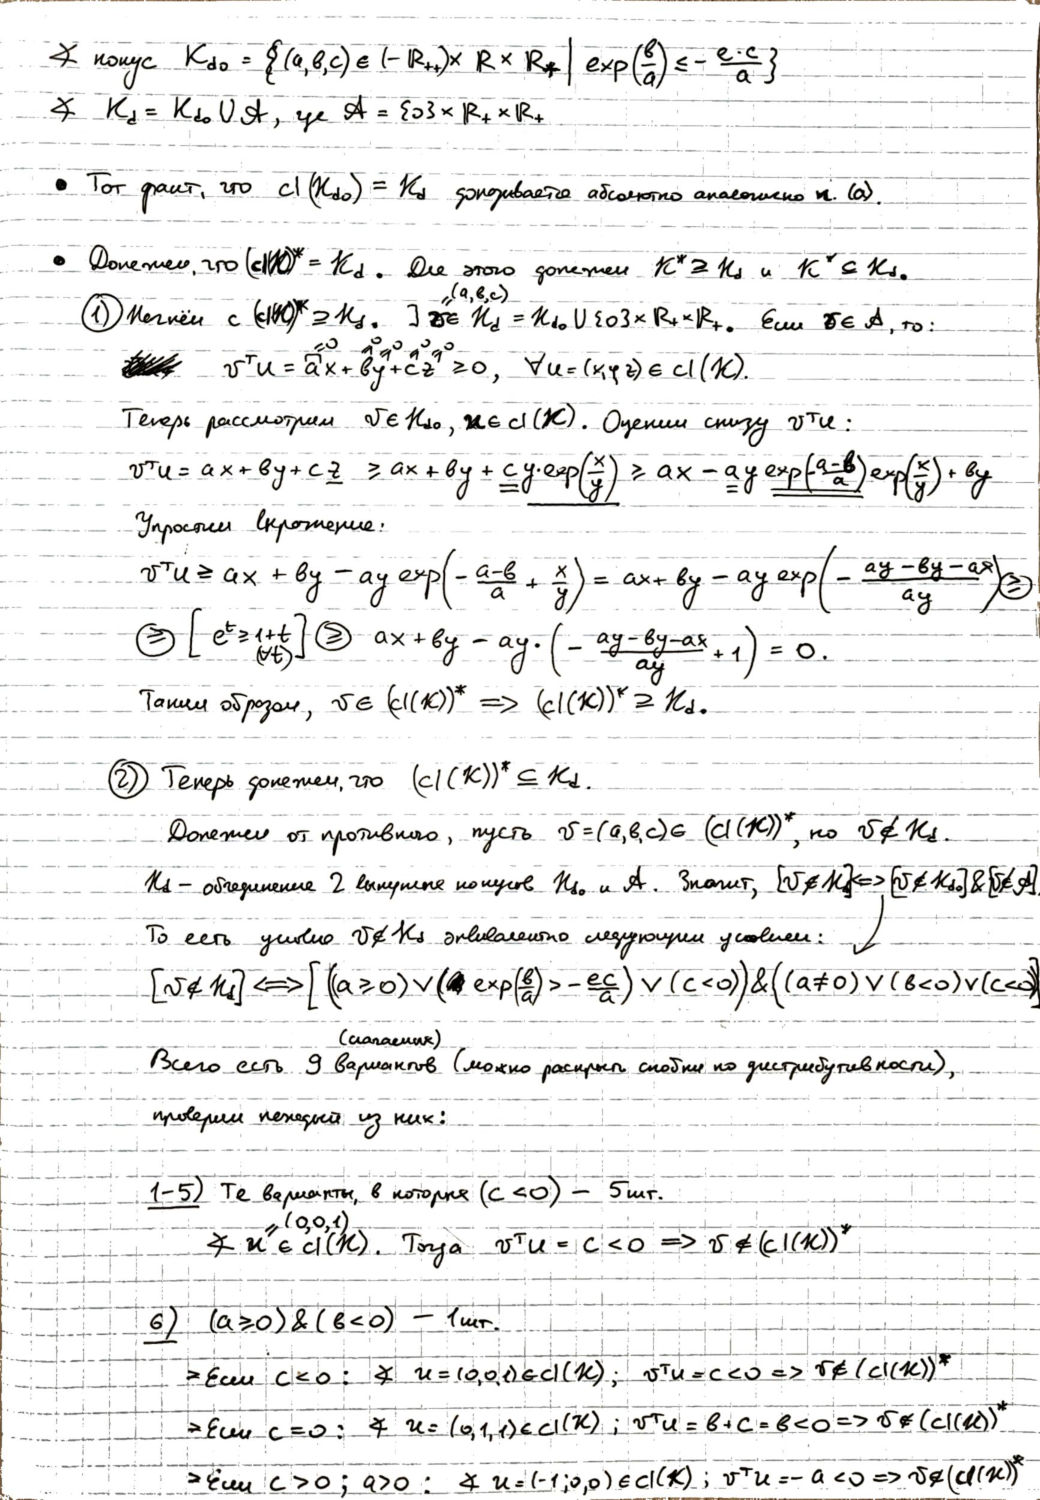
\includegraphics[width=0.82\linewidth]{figures/cone_1}
	\end{figure}
	\newpage
	\begin{figure}[h!]
		\centering
		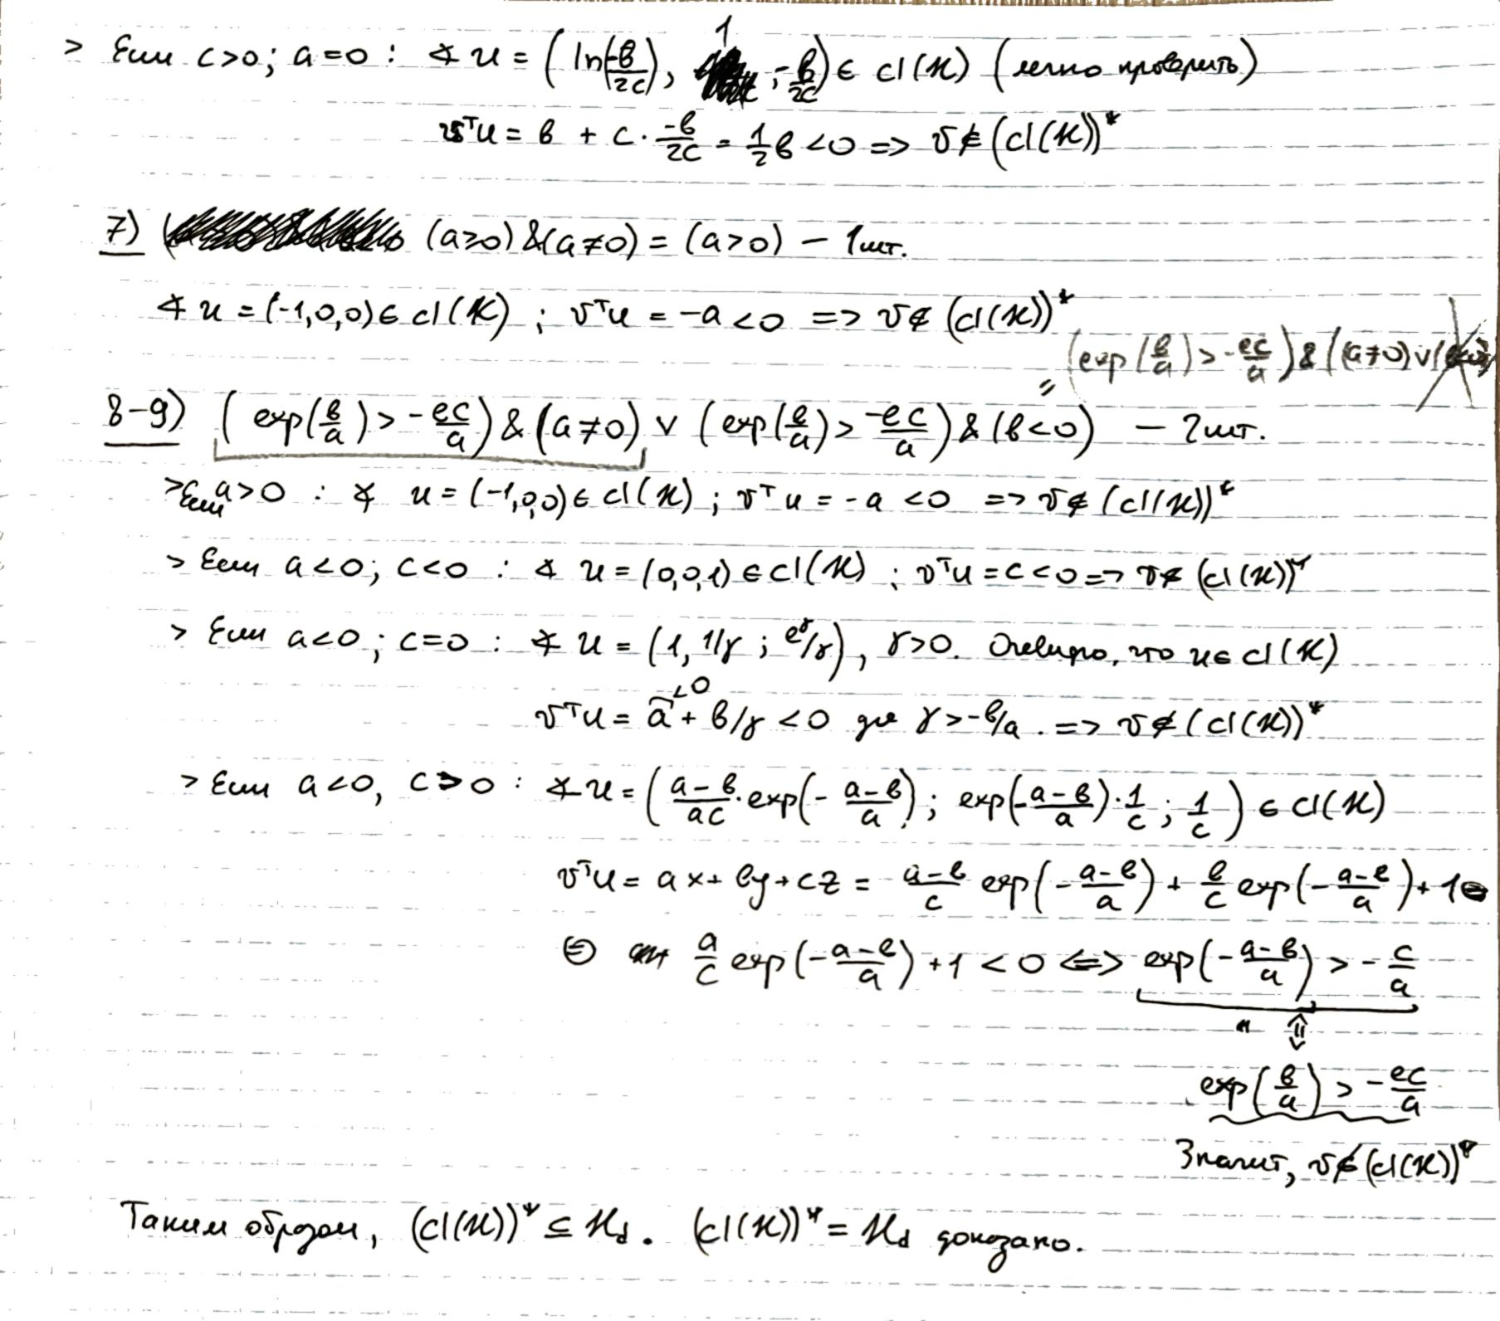
\includegraphics[width=0.82\linewidth]{figures/cone_2}
	\end{figure}
	
	
\end{document}